% Este archivo es parte de la memoria del proyecto fin de carrera
% de Diego Barrios Romero. Protegida bajo la licencia GFDL.
% Para más información, la licencia completa viene incluida en el
% fichero fdl-1.3.tex

% Copyright (C) 2012 Manuel López Urbina

\chapter{Organización temporal}
\label{chap:organización-temporal}

Para el desarrollo de OpenTSR ha sido necesario emplear varias herramientas, utilidades y bibliotecas. Algunas de ellas, ya habían sido utilizadas en ciertas ocasiones a lo largo de la carrera. Sin embargo, otras han requerido un periodo de formación previo, en el que se han adquirido los conocimientos necesarios para poder desarrollar el proyecto.\\

La mayor parte del proceso de investigación fue dedicado al estudio de las diferentes tecnologías existentes para el procesamiento de imágenes. Se comenzó realizando diferentes prototipos funcionales con Matlab, que además de ser un software privativo, no ofrecía la posibilidad de procesamiento de vídeo en tiempo real debido a su escasa velocidad de cálculo.\\

Posteriormente, tras la necesidad de solventar el problema de la velocidad, se optó por elaborar código con la alternativa libre a Matlab, Octave, implementando las funciones críticas en el lenguaje orientado a objetos C++. Resultando también insuficiente.\\

Continuando con las labores de investigación descubrí una biblioteca de uso muy extendido en robótica llamada OpenCV disponible en C, C++ y Python, resultando la disponible en C especialmente rápida en sus cálculos y proporcionando las características deseadas a las necesidades del proyecto, sobre todo la de dotar al sistema de la capacidad cálculo en tiempo real.\\

Todo ello ha implicado un tiempo bastante considerable en el uso, aprendizaje e investigación de las diferentes tecnologías existentes y comprobar su potencial.\\

Una vez decidida la herramienta para el procesamiento de imágenes, se consideró necesaria la idea de implementar una interfaz acorde con el sistema que permita el visionado de resultados al usuario y el entorno por el que se desplaza el vehículo. Para ello se utilizó la biblioteca Qt escrita en C++. Por tanto fue necesario tiempo para adquirir las nociones básicas de la biblioteca con la ayuda del entorno de desarrollo QtCreator.\\

Por otro lado, existen multitud de algoritmos y técnicas propias del reconocimiento de patrones que no son estudiadas durante la Ingeniería Técnica en Informática y que sí son vistas en la Ingeniería Informática añadiendo la necesidad de estudios de los conceptos propios del reconocimiento de patrones. Todo ello me ha supuesto un esfuerzo de investigación y aprendizaje bastante considerable.\\

Una vez determinadas las diferentes herramientas a utilizar se comenzó con la implementación de los diferentes prototipos funcionales para el software de reconocimiento de imágenes. Finalizado el software de reconocimiento se elaboró el sistema de comunicaciones con el vehículo y la interfaz gráfica.\\

La figura \ref{gantt:tareas} muestra una visión de las diferentes tareas desarrolladas para la elaboración del proyecto junto con la descomposición de cada una de ellas:\\

\begin{figure}[H]
  \begin{center}
    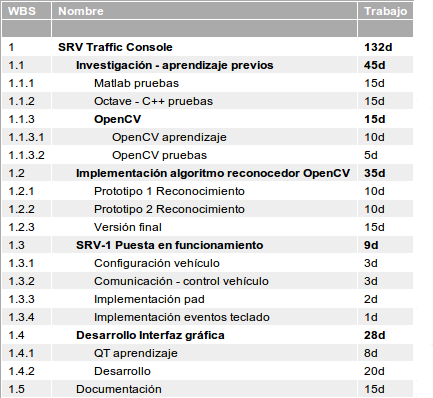
\includegraphics[scale=1]{tareas-gantt.png}
  \end{center}
  \caption{Descomposición de las tareas implicadas en el desarrollo del proyecto.}
  \label{gantt:tareas}
\end{figure}


\figura{gantt-1.png}{scale=0.5}{Diagrama de Gantt 1. Desarrollo del
  proyecto.}{gannt}{H}

\figura{gantt-2.png}{scale=0.5}{Diagrama de Gantt 2. Desarrollo del
  proyecto.}{gannt-2.png}{H}

\figura{gantt-3.png}{scale=0.5}{Diagrama de Gantt 3. Desarrollo del
  proyecto.}{gannt-3.png}{H}
